\chapter{Results and Discussion}
In this section the best models' capabilities are tested and discussed. Up to this point the model has been evaluated on labeled data, providing a clear ground truth to evaluate the models' predictions on. In this chapter the model will instead make predictions on unlabeled data and instead output its confidence in its prediction. We then discuss various topics with regards to the results found and some overall considerations.

\section{Real and Artificial Transition Regions}

While we previously mainly have focused on \gls{loo} accuracies, we have not in detail studied what the neural network softmax output that we base our classification on looks like. We are specifically interested in examining how well performance is when the robot moves across a \emph{transition region}, a region where the surface type changes from grass to non-grass and vice versa. Ideally the prediction should rapidly change according to the new target surface. 

This can be accomplished in two different ways. The first revolves around creating a test set through concatenation of sequences of radar sweeps from a few different data matrices. By selecting alternating surface types, we artificially generate transition region data which we can predict on. Examining these predictions we get a feel for what output the predictor could generate when moving from one surface to the next. The second method is to use real-world measurements from when the robot moves from one surface to the next. We should see that when the robot has reached the transition the prediction changes accordingly. 

\begin{figure}[t]
	\centering
	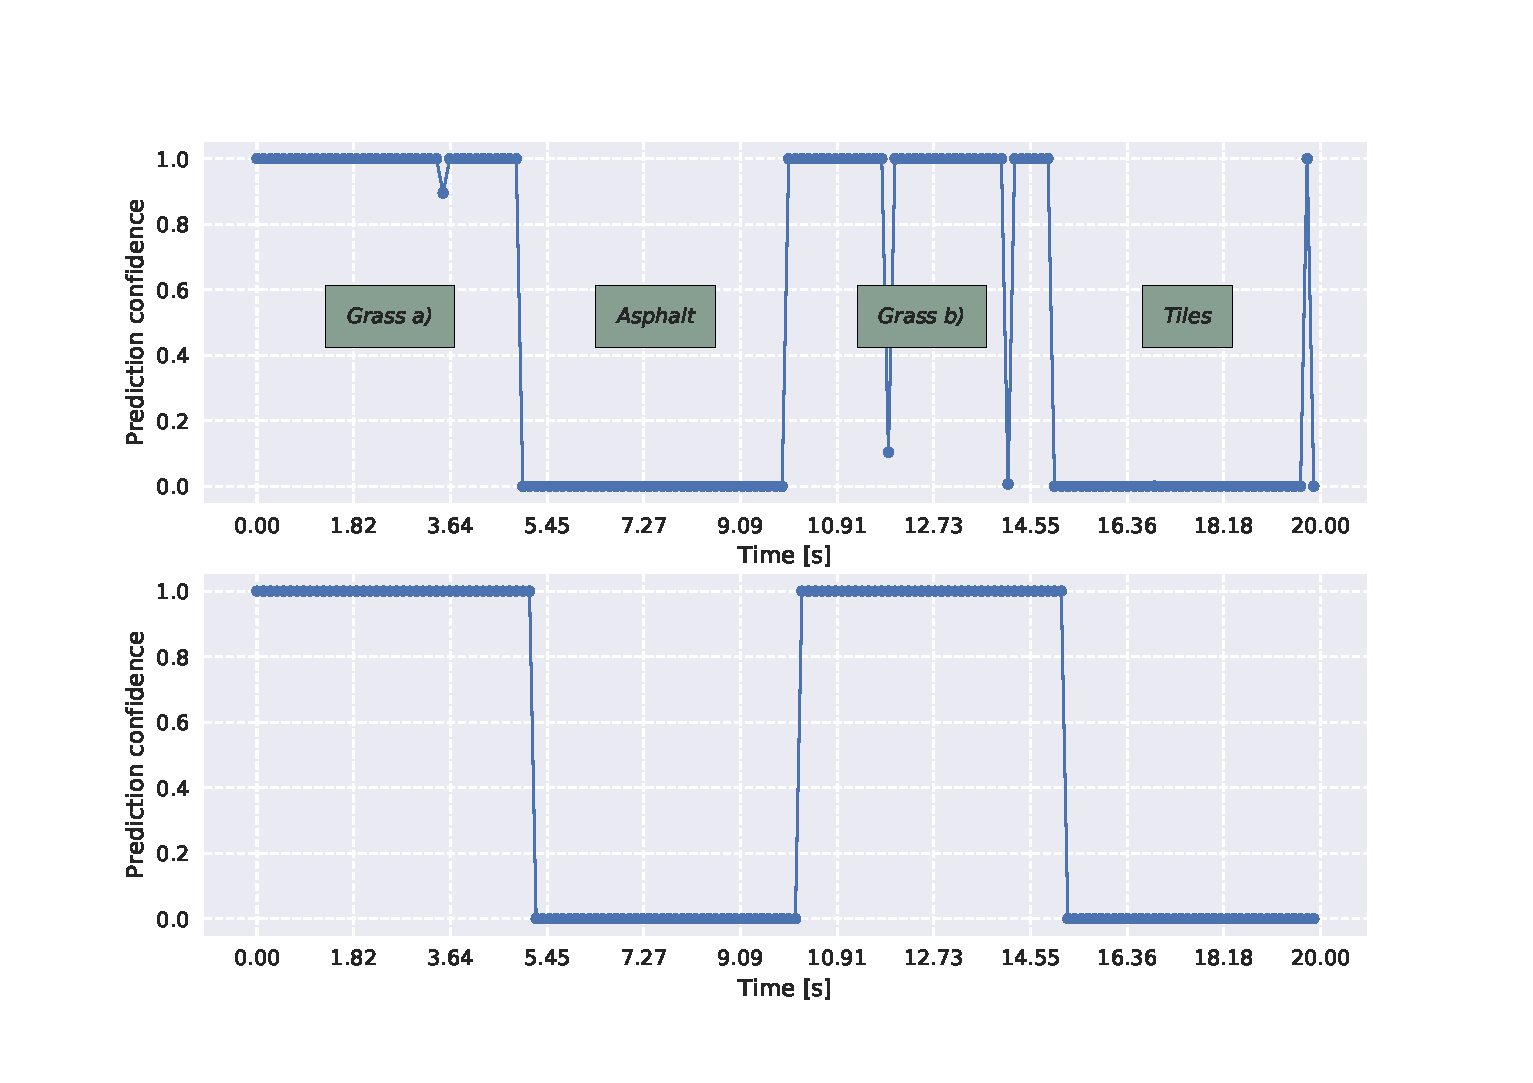
\includegraphics[scale=0.5]{figs_temp/varmats1}
	\caption{Predictions on an artificial transition region created using samples from four different regions. The bottom figure shows the median filtered predictions with filter length $L=5$.}
	\label{fig:artificial1}
\end{figure}

\begin{figure}[t]
	\centering
	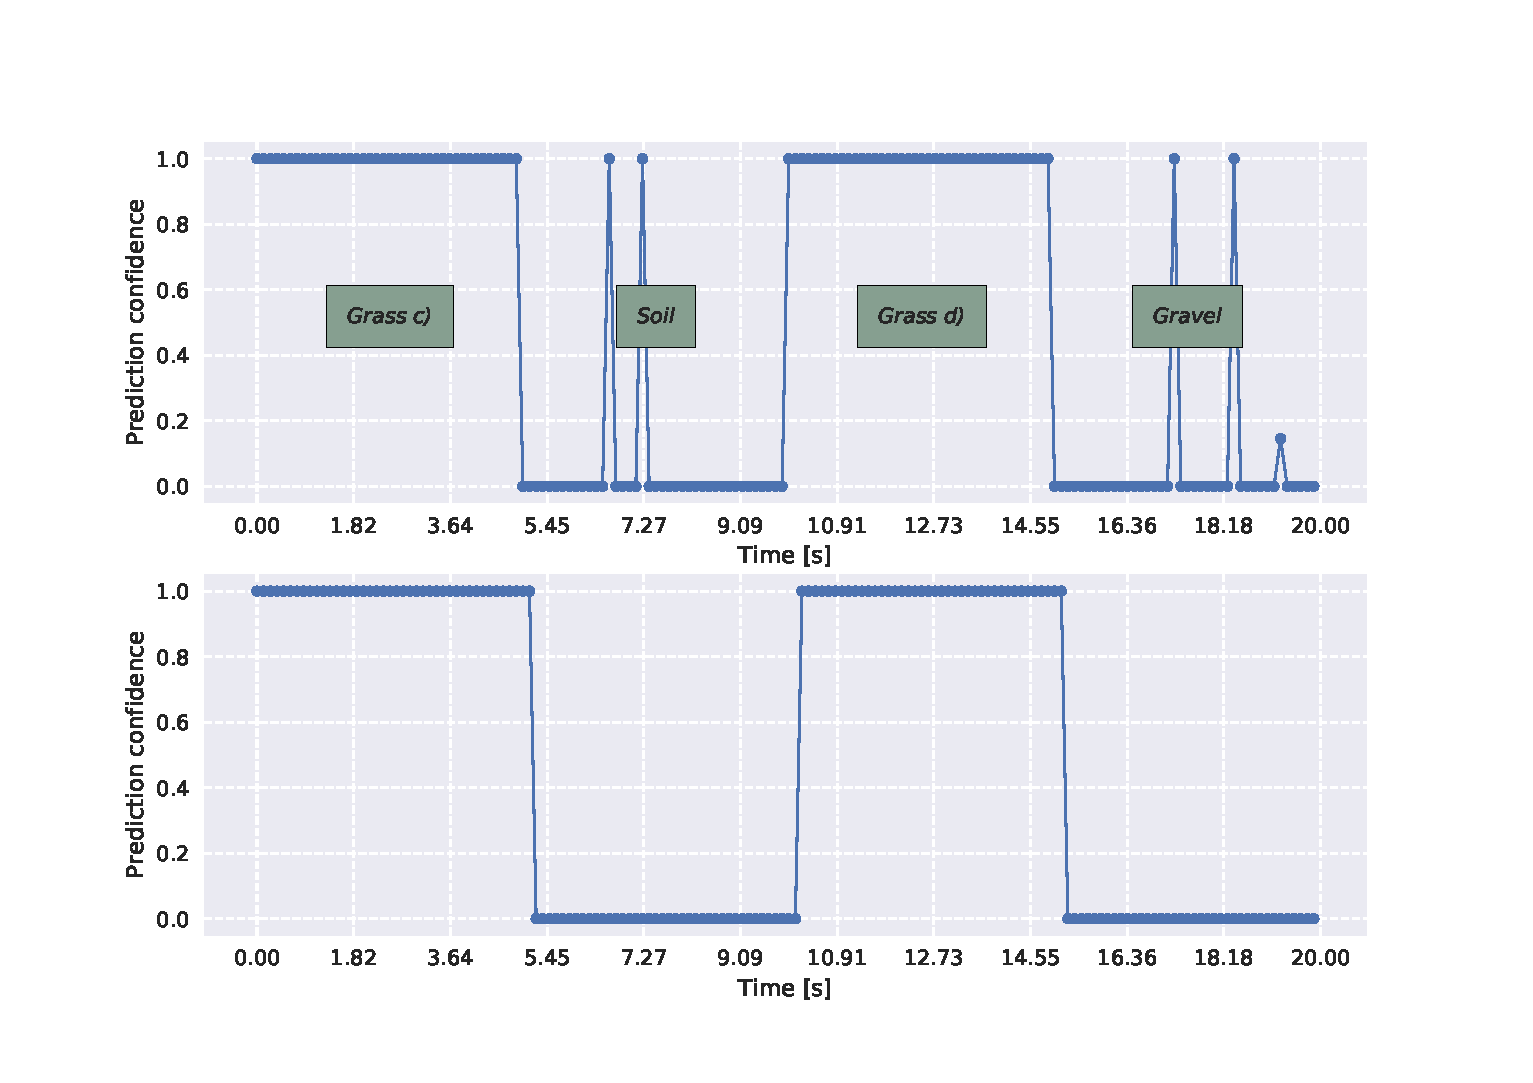
\includegraphics[scale=0.5]{figs_temp/varmats2}
	\caption{Predictions on an artificial transition region created using samples from four different regions.}
	\label{fig:artificial2}
\end{figure}

In the first test, samples from four surfaces are concatenated into a sequence: grass, asphalt, grass and tiles, where the two grass samples were taken from different data matrices. The predictions are shown in the top part of figure \ref{fig:artificial1}. In the lower part of this figure, the predictions are median filtered with filter length $L=5$ as was discussed in section \ref{surface_change}. The outliers are suppressed, rendering accurate predictions of the different surfaces. 

Two more challenging surfaces, according to table \ref{tab:loo}, are soil and gravel. In figure \ref{fig:artificial2} predictions on artificial transitions including these are shown. Something worth noting in the two figures is that the surface transition is delayed by two steps after the median filtering. It is important to be aware of what distance this corresponds to in the physical world, since we do not want to detect an edge too long after it has already passed. Each prediction uses 25 samples, and with a delay of two predictions this means a 50 sample delay. With the sampling rate at 200 Hz (see table \ref{tab:sensor_settings}), this means a 0.25 second delay in the edge detection, which for a robot traveling at the speed of $v=0.3$ m/s means a spatial delay of $0.3\cdot0.25=0.075$ m. This distance may be reduced by increasing the classification rate. This could of course be done by altering $T$ or $F_s$ in \eqref{eq:classification_rate}, but also through making predictions more frequently by allowing the model to make a prediction at intermediate points, given the $T$ \emph{most recent} sweeps.

Looking at the high \gls{loo} accuracies in table \ref{tab:loo}, the results of classifications upon the artificial transitions should not come as a surprise, as they are based on the same data. What can be seen that we didn't know from table \ref{tab:loo} is that not only does the model classify correctly, but usually  does so with a very high confidence. 

To test the model further, data was collected when the test robot moved from one surface to another. Figure \ref{fig:trans_tgtg} shows a transition from grass to tiles, and figure \ref{fig:trans_gg} a transition from grass to gravel. Focusing on the median filtered predictions, we see that outside the transition region, the model works well for classifying either surface. Looking at the transitions sections, we see a rather sharp switch in prediction confidence. Nonetheless, this switch is not immediate. This is likely due to that the wide combined field of view of the two sensors captures both regions simultaneously, and thus the model tries to make a prediction on data obtained from a mixture of the two surface types. 

% I think this explanation is overly long
%What happens around the transition is perhaps more interesting. In the previous figures, the predictions went from 1 to 0 and vice versa in just one step. Here, it takes a while before the model reaches zero-outputs. There are two possible explanations for this. First of all, in the artificial transitions, the surface went from a perfect grass surface to a perfect non-grass surface at an instance. In real transitions, there might be some overlap of grass on the non-grass surface, making the model unsure of what it sees. Another explanation could be that one sensor is facing straight down, whereas the other one looks slightly more forward. Hence, the model is perceiving both grass and tiles simultaneously during a short time. 

% ?
%The results show great promise, but the work is still at an early stage. The surfaces in the four transitions were intentionally free from as many obstructions as possible. When facing surfaces with characteristics not taken into regard by the model, the results will not likely be as good. 
\begin{figure}
	\centering
	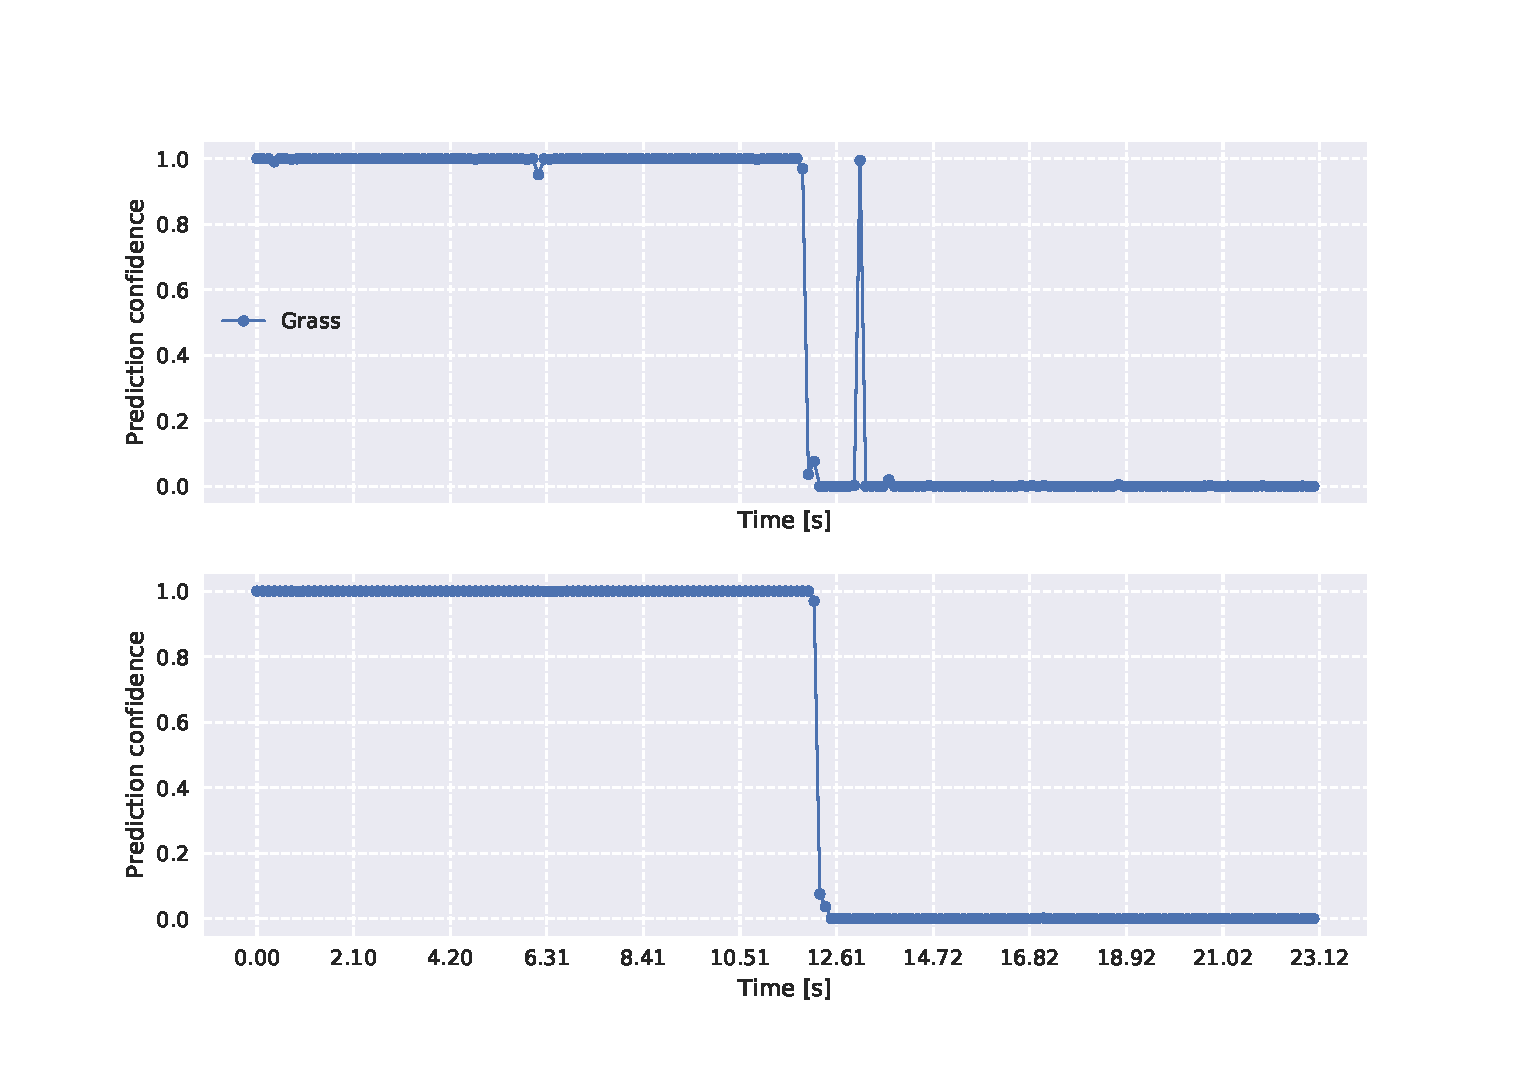
\includegraphics[scale=0.5]{figs_temp/transition_grass_tiles_grass}
	\caption{Predictions from a real-world test where the robot moved from grass to a tiled pavement.} 
	\label{fig:trans_tgtg}
\end{figure}

\begin{figure}
	\centering
	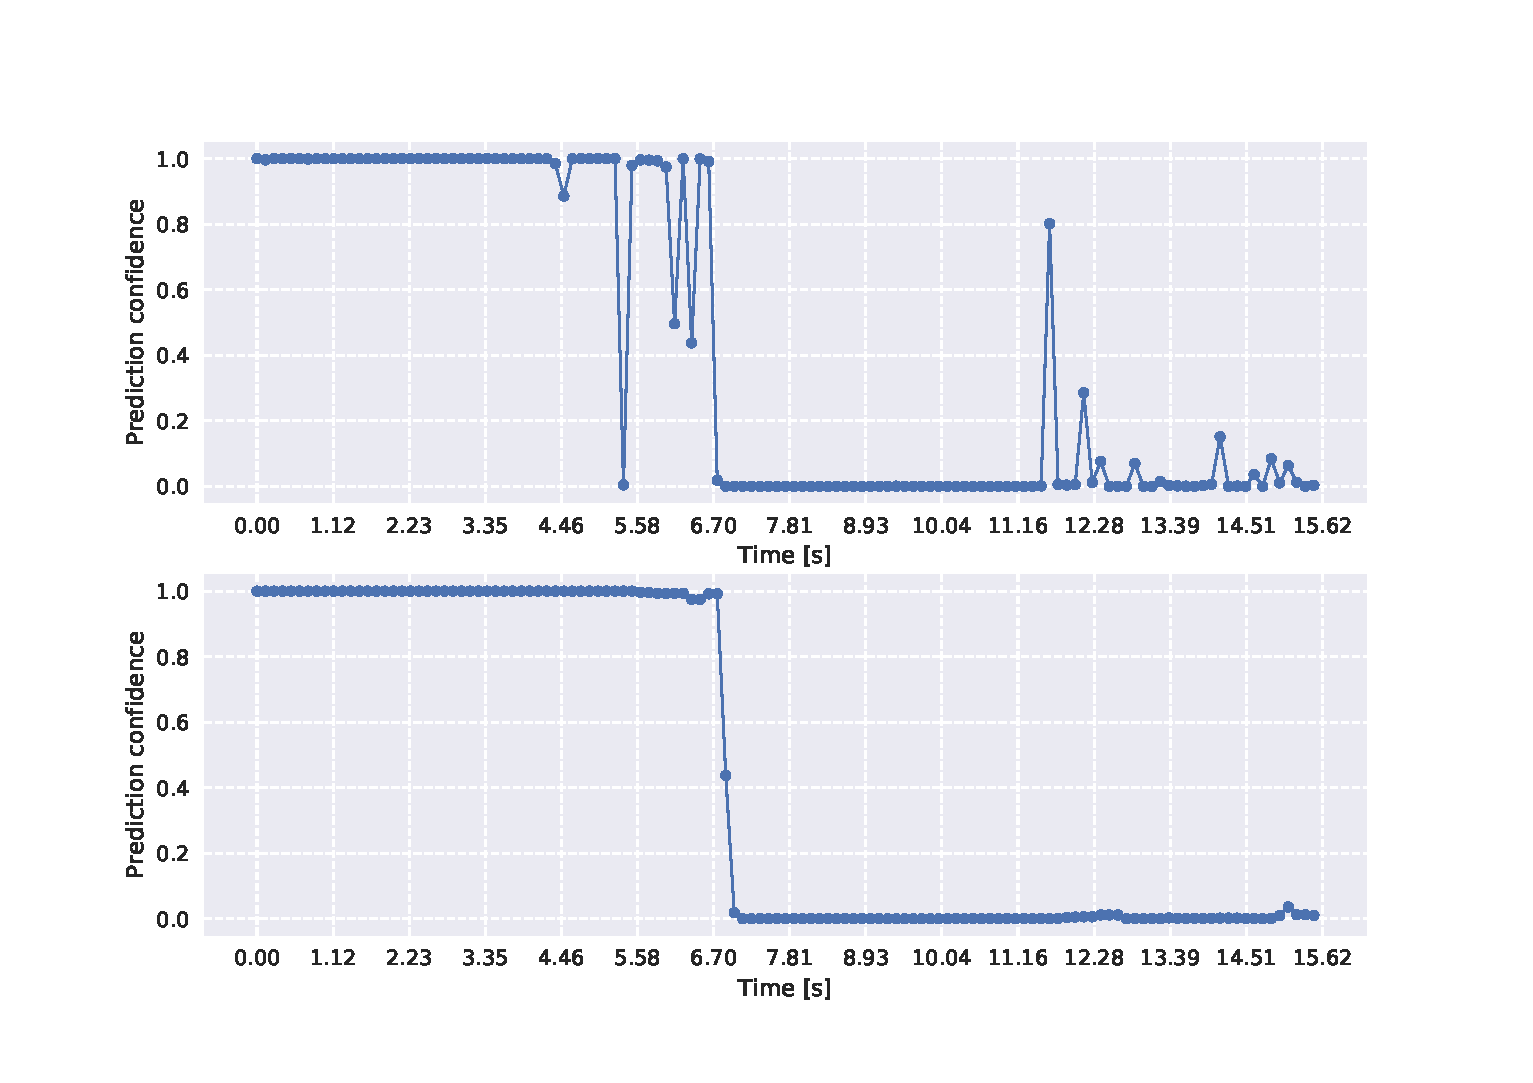
\includegraphics[scale=0.5]{figs_temp/transition_grass_gravel2}
	\caption{Predictions from a real-world test where the robot moved from grass to gravel.}
	\label{fig:trans_gg}
\end{figure}

\section{Surface Variances}

One particularly challenging aspect of adequately classifying surfaces is that the space of realistically occurring surface variations is essentially infinite. As any lawn owner can testify a lawn changes drastically over the course of its life span depending on grass height, weather conditions, tear and temperature. One would certainly need an enormous training dataset to capture all such variations. And that would still only account for one single lawn. It wouldn't take much for the classifier to enter uncharted territory, as the machine learning classifier solely bases its predictions on training feature vectors.

However, we see from our results that accurate classification is possible when acquired data is reasonably similar to what has been seen in training. A robot \emph{can} learn to identify surfaces as being grassy or not provided that it has previously been exposed to somewhat similar surfaces before. 

To remedy for the dangers of using an unchecked neural network classifier one should consider using some supporting sanity-check system in conjunction with the algorithm suggested in this thesis to improve robustness. Checking that returning signals are of reasonable strengths or that the distance to the ground remains unchanged are suggestions.


%In some cases, the robot may even come across surface types unlike any it has ever seen before. It is difficult to foresee what a complex neural network will make of this and it will exhibit an unpredictable behaviour. 
%%%%%%%%%%%%%%% Introduce again when we actually have done it.
%\section{Difficult Surfaces}


%While we only have five material classes in this work, each class can be broken down to multiple subclasses. Taking grass as an example, it may vary in a wide range of attributes such as length, humidity and sparsity to name a few. Therefore it is important to gather a dataset as diverse as possible, so that the model has trained on all common varieties of each surface. 

%However, the model can only be prepared for so much, and an often critical aspect of any machine learning system is its performance on dissimilar data. It is difficult to foresee how a complex neural network will interpret a surface displaying characteristics not included in training. For instance, what would the model make of a lawn which is partially covered by leaves and twigs; or a surface type it has never seen before? Perfecting the model to work in any surrounding calls for a good sense of what difficulties may occur, as well as a large time investment. 




%\section{Moisture}

%One particularly challenging aspect of adequately classifying surfaces is the ever-changing environmental conditions surronding the sensor. Of particular interest is the moisture content in the surfaces of interest. Greater soil moisture implies higher dielectric constant, which in turn increases radar wave scattering \citep{rappaport_2006}. Thus a single surface may very well change its scattering properties over time. 

% More things that make selecting data tricky

%\section{Surface variances}


%Such effects is difficult to account for when selecting data. Gather a dataset as diverse as possible



\section{Feature Extraction and Model Selection}
\label{disc_feat}
Table \ref{tab:loo} is in many ways a very telling one. Using the \gls{loo} cross validation strategy each data measurement was classified without using any of the samples from the measurement session the data was taken from. Six different methods of classification were evaluated; two linear and four nonlinear. 

First and foremost it is noted that each tested method performed at the very least \emph{decently}. One may argue that the \gls{lstm} model is unstable or that using \gls{lda} produces lower accuracy predictions, but they nonetheless generated average accuracies above 97\%. Considering that these are the lower-performing classifiers and the remaining ones perform even better suggests that the performed feature extraction captures, or at least maintains, most of the crucial information in the original data. The \gls{pca}-plot in figure \ref{fig:pca} served as a proof of concept to this already at an early stage, as some degree of separation can be seen in only two dimensions. Furthermore, as linear models managed to separate data decently we know that the information content is readily available without the usage of more advanced non linear classifiers.  

A deep learning puritan might argue that no feature extraction should be performed when working with deep neural networks; a network should be able to find good data characteristics on its own. Hence, an \gls{ann} may yield a better result by omitting the feature extraction process as this unavoidably discards some information in the original data. 

Since much of the information needed to distinguish grass from non-grass surfaces is in the slow time dimension a neural network needs to be exposed to multiple sweeps to extract such information. This can either be done through concatenation of a several sweeps, or through some version of a recurring neural network. The first option is computationally expensive, as the network needs to figure out how to compute useful features from the set of complex data matrix which certainly would require a deep neural net. The second was investigated in this report through the \gls{cnn} and \gls{lstm} model from \citep{karim_majumdar_darabi_chen_2018}. While it for many surfaces did perform very well, it showed lackluster performance on others indicating poor robustness, while simultaneously being the most complex of the investigated models. It may nonetheless be of interest to investigate if robustness can be improved for this model. However, based solely on the results found in this report we argue that the reduced complexity and increased control makes the feature extraction process worthwhile for the task of distinguishing grass from non-grass surfaces.  

%However, since much of the information seems to be found in how signals evolve over time, a network with no feature extraction would require multiple sweeps to be concatenated into one feature vector in order to be able to find these time dependencies. Say it would take 25 (downsampled) sweeps, each with 14 range bins. Each sweep would then produce 28 features as the real and imaginary part are divided into separate features. The feature vector to such a network for two sensors with different mounting angles would then consist of $2\times25\times28=1400$ features. Furthermore the network would have to figure out all the complex-valued temporal processing techniques that we already know how to calculate from theory. So although using no feature extraction method whatsoever could \emph{potentially} increase accuracy with a large \gls{dnn} model, we argue that the added complexity and reduced control is a high price to pay for this increase. 

On a different note, the final choice of classifier is debatable. The \gls{dnn} classifier was chosen mainly due to its high stable \gls{loo} scores in table \ref{tab:loo}. Nonetheless linear models performed well too, but didn't quite reach the accuracies of the \gls{dnn} model, implying that the features are at least \emph{approximately} linearly separable. Placing more effort on the linear models through testing more types of linear classifiers and optimizing their hyperparameters more carefully might make one of the linear models the top choice.

%The \gls{lstm} approach showed great promise with its leading median \gls{loo} score. However, its occasional dips in performance lowered the mean score, making it less desirable. The reason behind these dips is unknown. While we only tested the basic model in \citep{karim_majumdar_darabi_chen_2018}, they do describes an extension of the model that is supposedly better at learning long term dependencies in long sequences. It is possible that the extended model would better our results, but as there is no mention in the article of what is regarded as a long sequence and our sequences hold merely 25 samples. Therefore we chose to not examine the extended model.

\section{Errors and Uncertainties}
For this project a total of 42 data matrices were captured from 5 different surface types, see table \ref{tab:count}. The number of matrices acquired from each surface was based on having a reasonably balanced dataset with a similar number of grass and non-grass samples. Having a balanced (or near-balanced) measurement set ensures that the classification is not biased either way; with more samples of one class the classifier will naturally tend towards the surface type it has seen more of in training. This however leaves other surfaces with less similar training data, and it is well possible that more measurements of the lower-performing soil and gravel surfaces are needed.  

% I think this is weirdly written
%But the question of what a balanced dataset \emph{is} sometimes holds multiple answers. In this work, there are four different types of materials belonging to class 0 (not grass) and one belonging to class 1. A natural question to ask oneself is whether there should be equally many samples for each \textit{material}, or equally many for each \textit{class}. We have chosen to balance the dataset so that there are approximately as many samples in each class. If all grass surfaces looked the same, this would perhaps make the model biased in its predictions, but due to the great variety among grass surfaces the bias is eliminated.

Another risk when collecting data is obtaining too little of it. By looking at how little improvement the data augmentation made in table \ref{tab:aug}, it would seem that obtaining $Q=50,000$ sweeps per data matrix was enough. However by increasing the number of data matrices collected we increase \emph{data diversity}, capturing a wider range of grass types. 

A more technical uncertainty regards the assumption of a constant velocity over different surfaces. The robot used in this project kept a somewhat steady pace regardless of surface type, but when faced with rough terrain or steep hills the robot's velocity altered a fair bit. As both the \gls{dft} and autocovariance require a consistency in the spacing between sample points, we cannot tolerate too large variations in velocity. Hence, to sample at regular distances the sampling could be controlled by positional feedback from the robot rather than a fixed sampling frequency.

Previously we mentioned that predictions can be made more frequent by continuously keeping track of the $T$ most recent samples. A similar idea can be applied to the normalization process. Even if we only use $T=25$ sweeps for feature extraction, we are not limited to use only those for the sweep normalization. By in addition using sweeps from further back in time, a more stable mean energy estimate is achieved. The estimate could in theory be updated for each new sample.

% TODO: I think this should either be moved to future work or not included
% While this work has not put much focus on \textit{live} classifications, this does pose a new limitation on the model. Ideally we want the system to collect $T$ samples, and make an instantaneous prediction so that $T$ new samples can be collected right away. By running the system on a single thread, however, the time it takes to generate a prediction delays the data collecting process with some time $t_{cl}$, as only one process can be ran at a time. An alternative could be to handle the classifications in a separate thread. That way, data could be collected continously, while classifications are performed in parallel. Doing this requires caution. If the time it takes to generate a classification exceeds the time it takes to collect $T$ samples, i.e. $t_{cl}>T/F_s$, a delay will accumulate over time. After a while predictions would be irrelevant as they would be based on surfaces far behind the robot. A natural limitation to assign the model is therefore
%\begin{equation}
%	t_{cl} \le \frac{T}{F_s}.
%\end{equation}
%The time $t_{cl}$ has not been discussed in this work, but is highly relevant to study in the future.



% This remarkable result means that given a random sample from the dataset collected, with no samples from the session the sample was taken from used in training, we can correcly classify the surface as grass or non-grass 39/40 times even with the lower-performing classifiers. With the top performing fully connected model, even higher accuracy was obtained with a low standard deviation. 


